\documentclass[11pt,letterpaper]{article}

\makeatletter
\renewcommand\paragraph{\@startsection{paragraph}{4}{\z@}%
                                      {1ex \@plus1ex \@minus.2ex}%
                                      {-1em}%
                                      {\normalfont\normalsize\bfseries}}
\makeatother

%%%%%%%%%%%%%%%%%%%%%
%  P A C K A G E S  %
%%%%%%%%%%%%%%%%%%%%%

% Authors
\usepackage{authblk}

% Page margins
\usepackage[margin=1in]{geometry}

% Nicer math font
\usepackage{mathpazo}

% More fancy lists
\usepackage{enumerate}

% Microtype
\usepackage{microtype}

% TikZ
\usepackage{tikz}
%\usetikzlibrary{calc,shapes.geometric}
\usetikzlibrary{backgrounds,fit,decorations.pathreplacing,calc}

% Highlights
\usepackage{soul}


% Figure
\usepackage{float}

% Hypertext package
\usepackage[colorlinks = true]{hyperref}
% Title and authors
%\hypersetup{
%  pdftitle = {},
%  pdfauthor = {}
%}
% Color definitions
\definecolor{darkred}  {rgb}{0.5,0,0}
\definecolor{darkblue} {rgb}{0,0,0.5}
\definecolor{darkgreen}{rgb}{0,0.5,0}
% Color links
\hypersetup{
  urlcolor   = blue,         % color of external links
  linkcolor  = darkblue,     % color of internal links
  citecolor  = darkgreen,    % color of links to bibliography
  filecolor  = darkred       % color of file links
}

% AMS
\usepackage{amsmath,amssymb,amsfonts,amsthm,amstext}

%% Restating theorems
%\usepackage{thm-restate}

% Powerful macros
\usepackage{etoolbox}

% Fixes for amsmath
\usepackage{mathtools}
\mathtoolsset{centercolon}
\makeatletter
\protected\def\tikz@nonactivecolon{\ifmmode\mathrel{\mathop\ordinarycolon}\else:\fi}
\makeatother

% Daw boxes
\usepackage{tcolorbox}

% Code
\usepackage{algorithm}
%\usepackage{algorithmic}
\usepackage{algpseudocode}

% Clever references

\usepackage{cleveref}%[nameinlink]


\crefname{lemma}{Lemma}{Lemmas}
\crefname{proposition}{Proposition}{Propositions}
\crefname{definition}{Definition}{Definitions}
\crefname{theorem}{Theorem}{Theorems}
\crefname{conjecture}{Conjecture}{Conjectures}
\crefname{corollary}{Corollary}{Corollaries}
\crefname{claim}{Claim}{Claims}
\crefname{section}{Section}{Sections}
\crefname{appendix}{Appendix}{Appendices}
\crefname{figure}{Fig.}{Figs.}
\crefname{table}{Table}{Tables}


% \crefname{algorithm}{Algorithm}{Algorithms}

% IEEE tools
\usepackage[retainorgcmds]{IEEEtrantools}

% table of contents
\usepackage{tocloft}

% Table with multi-row
\usepackage{multirow}

% TikZ
\usepackage{tikz}	
\usetikzlibrary{backgrounds,fit,decorations.pathreplacing}

%%%%%%%%%%%%%%%%%%%%%%%%%
%  N E W C O M M A N D  %
%%%%%%%%%%%%%%%%%%%%%%%%%

% Standard quantum notation

\newcommand{\ket}[1]{|#1\rangle}
\newcommand{\bra}[1]{\langle#1|}
\newcommand{\braket}[2]{\langle#1|#2\rangle}
\newcommand{\ketbra}[2]{|#1\rangle\langle#2|}
\newcommand{\proj}[1]{|#1\rangle\langle#1|}

\newcommand{\x}{\otimes}
\newcommand{\xp}[1]{^{\otimes #1}}
\newcommand{\op}{\oplus}

\newcommand{\ct}{^{\dagger}}
\newcommand{\tp}{^\intercal}

% Linear algebra

%\newcommand{\1}{\mathbb{1}} % identity matrix
%\DeclareMathOperator{\Hom}{Hom}
\DeclareMathOperator{\End}{End}
%\DeclareMathOperator{\E}{\mathbb{E}}
\DeclareMathOperator{\Lin}{L} % all linear maps
\newcommand{\Mat}[1]{\mathrm{M}(#1)} % all matrices
%\newcommand{\Mat}[1]{\mathrm{M}_{#1}(\C)}

% Paired delimiters

\DeclarePairedDelimiter{\set}{\lbrace}{\rbrace}
\DeclarePairedDelimiter{\abs}{\lvert}{\rvert}
\DeclarePairedDelimiter{\norm}{\lVert}{\rVert}
\DeclarePairedDelimiter{\cnorm}{\lvert}{\rvert}
\DeclarePairedDelimiter{\of}{\lparen}{\rparen}
\DeclarePairedDelimiter{\sof}{\lbrack}{\rbrack}
\DeclarePairedDelimiter{\ip}{\langle}{\rangle}
\DeclarePairedDelimiter{\floor}{\lfloor}{\rfloor}

% Operators

\renewcommand{\Re}{\operatorname{Re}}
\renewcommand{\Im}{\operatorname{Im}}
\DeclareMathOperator{\vc}{vec}
\DeclareMathOperator{\spn}{span}
\DeclareMathOperator{\rank}{rank}
\DeclareMathOperator{\diag}{diag}
\DeclareMathOperator{\spec}{spec}
\DeclareMathOperator{\Tr}{Tr}
\DeclareMathOperator{\sgn}{sgn}
\DeclareMathOperator{\hook}{hook}
\DeclareMathOperator{\E}{\mathbb{E}}
\DeclareMathOperator{\supp}{supp}


% Sets

\newcommand{\C}{\mathbb{C}}
\newcommand{\R}{\mathbb{R}}
\newcommand{\N}{\mathbb{N}}
\newcommand{\Z}{\mathbb{Z}}
\newcommand{\calH}{\mathcal{H}}
\newcommand{\calX}{\mathcal{X}}
\newcommand{\calY}{\mathcal{Y}}
\newcommand{\calA}{\mathcal{A}}
\newcommand{\calB}{\mathcal{B}}

% Group
\newcommand{\Zd}{\Z_d^{\times}}


% Identity operator
\newcommand{\1}{\mathbb{1}}

% Pauli Group
\newcommand{\Pg}{\mathcal{P}}
\newcommand{\J}{\mathcal{J}}

% Special notation

\newcommand{\CHSH}{CHSH^{(d)}}
\newcommand{\MS}{MS}
\newcommand{\EXT}{EXT}
\newcommand{\LS}{LS}
\newcommand{\COMM}{COMM}
\newcommand{\EPR}[1]{\Sigma^{(#1)}}
\newcommand{\paulix}{\sigma_x}
\newcommand{\pauliz}{\sigma_z}
\newcommand{\tP}{\tilde{P}}
\newcommand{\tQ}{\tilde{Q}}
\newcommand{\tM}{\tilde{M}}
\newcommand{\tN}{\tilde{N}}
\newcommand{\tA}{\tilde{A}}
\newcommand{\tB}{\tilde{B}}
\newcommand{\tX}{\tilde{X}}
\newcommand{\tZ}{\tilde{Z}}
\newcommand{\tU}{\tilde{U}}
\newcommand{\tW}{\tilde{W}}
\newcommand{\tx}{\tilde{x}}
\newcommand{\tpsi}{\tilde{\psi}}
\newcommand{\tri}{\Delta}
\newcommand{\lB}{\overline{B}}
\newcommand{\dr}[1]{d^{(#1)}}
\newcommand{\nr}{n(r)}
\newcommand{\mr}{m(r)}
\newcommand{\ux}{\underline{x}}
\newcommand{\uc}{\underline{c}}
\newcommand{\ua}{\underline{a}}
\newcommand{\ub}{\underline{b}}
\newcommand{\fC}{\mathfrak{C}}
\newcommand{\ba}{\pmb{a}}
\newcommand{\bb}{\pmb{b}}
\newcommand{\bc}{\pmb{c}}
\newcommand{\bS}{\mathrm{S}}

% Probabilities
\newcommand{\pr}[2]{P(#1|#2)}
\newcommand{\pa}[2]{P_A(#1|#2)}
\newcommand{\pb}[2]{P_B(#1|#2)}
\newcommand{\tpr}[2]{\tilde{P}(#1|#2)}

% Bell Ineqaulities
\newcommand{\I}{\mathcal{I}}

% Square root of epsilon
\newcommand{\ep}{\epsilon}
\newcommand{\se}{\sqrt{\epsilon}}
\newcommand{\qe}{\epsilon^{1/4}}
\newcommand{\sd}{\sqrt{d}}
\newcommand{\sr}{\sqrt{r}}
\newcommand{\qr}{r^{1/4}}
\newcommand{\qd}{d^{1/4}}

% Approximately equatli
\newcommand{\appd}[1]{\simeq_{#1}}

% Comments
\def\carl#1{{\color{blue} #1}}
\newcommand{\hf}[1]{\textcolor{red}{#1}}
\newcommand{\hfc}[1]{\textcolor{red}{#1 -H.F.}}

%%%%%%%%%%%%%%%%%%%%%%%%%
%  N E W T H E O R E M  %
%%%%%%%%%%%%%%%%%%%%%%%%%

\newtheorem{theorem}{Theorem}
\newtheorem{lemma}[theorem]{Lemma}
\newtheorem{proposition}[theorem]{Proposition}
\newtheorem{definition}[theorem]{Definition}
\newtheorem{corollary}[theorem]{Corollary}
\newtheorem{conjecture}[theorem]{Conjecture}
\newtheorem{claim}[theorem]{Claim}
\newtheorem*{conjecture*}{Conjecture}
\newtheorem*{problem}{Problem}
\newtheorem*{example}{Example}

\theoremstyle{definition}
\newtheorem*{remark}{Remark}



%%%%%%%%%%%%%%%%
%   Document   %
%%%%%%%%%%%%%%%%
\vspace{-8ex}
\date{}
\begin{document}

\title{Constant-sized correlations are sufficient to 
robustly self-test maximally entangled states with unbounded dimension}

\author{Honghao Fu}

\maketitle

The certification of a quantum device is an important building block
for many quantum information processing tasks, especially
when the devices are provided by some untrusted vendor.
We would like such certification to be done based solely on
the observed measurement statistics with the only assumption being that
any local device cannot communicate their own
inputs to the other local devices. 
The measurement statistics are referred to as correlations.

It has been shown that certain quantum correlations require the distant parties to share
a particular entangled state up to some local isometry. 
This phenomenon is referred to as self-testing.  
If we can further prove that, when the observed correlation deviates from 
the ideal correlation to some extent, 
the shared state is close to the ideal state up to some local isometry,
then we say the self-test is robust. 

Self-testing is powerful because only classical interactions are performed.
Hence, it allows a classical party to delegate quantum computation tasks to some untrusted service provider
and verify that the computations are performed
honestly and correctly \cite{ruv2013,coladan2017verifier}.
It also becomes a critical component of the security proofs of device-independent quantum cryptographic protocols
\cite{mayersyao,vv2014,miller2017,fu2018,eat2018}.
Since the setting of interactive proof systems is similar to a self-test, self-testing arguments also help to prove
lower bounds of the computational power of entanglement-assisted
multiprover interactive proof systems \cite{fitzsimons2019, neexp}.


Robust self-testing of the EPR pair, 
$\ket{EPR} = \frac{1}{\sqrt{2}}(\ket{00}+\ket{11})$,
is first proved in \cite{mckague2012}, then 
the techniques are improved in \cite{bamps2015}.
Robust self-testing of partially entangled qubits is later proved in
\cite{yang2013}.
Robust self-testing results of tensor product of maximally and partially entangled qubits 
are proved in \cite{coladan2016parallel,natarajan2017,lowdegree},
with the last one being the one with the smallest input and output alphabet.
For general bipartite entangled quantum states, \cite{coladan2017all} proves that there exists a family of correlations such that
each bipartite entangled state can be self-tested by a correlation in this family.
% The authors constructed a family of correlations such
% that each partially or maximally entangled state of any local dimension has
% a self-testing correlation in this family.
% One can also self-test many copies of the $2$-dimensional EPR
% pair in parallel \cite{mckague2016,natarajan2017,coladan2016parallel}.
% The most efficient way uses $O(\log n)$ bits question and
% answers to self-test $n$ copies of $2$-dimensional EPR
% pair \cite{lowdegree}.
% Self-testing general $d$-dimensional EPR pairs is a harder task.
% Coladangelo, Goh and Scarani has shown that all pure bipartite entangled states can be self-tested \cite{coladan2017all}


There are two open questions about self-testing that we aim at answering.
The first one is whether maximally entangled states with large local dimension
can be self-tested with constant-sized input and output alphabets. 
For comparisons,
all the self-testing correlations used in the results listed above have 
output alphabets with size depending on $d$
when they try to self-test an entangled state of local dimension $d$.
The second one is how to robustly self-test maximally entangled states
with local dimension $d > 2$ and $d \neq 2^n$ for any $n$.
For example, the authors of \cite{coladan2017all} left proving their
family of self-testing correlations robust as an open problem.

We give an affirmative answer to the first question
and make significant progress in answering the 
second question
by proving the following theorem.  
\begin{theorem}[Informal]
\label{thm:inf}
	There exists an infinite-sized set $D$ of odd prime numbers such that, for any $d \in D$, 
	the maximally entangled state of local dimension $4(d-1)$ can be robustly self-tested 
	with constant-sized input and output alphabets.
\end{theorem}
Formal statements of this theorem can be found in Theorem $6.16$ and $6.17$
of the attached report.
% The formal statement of this theorem is given in \cref{thm:self-test} and \cref{thm:infty}.

\textbf{Sketch of the proof}.
The set $D$ is, specifically, the set of all 
odd prime numbers whose smallest primitive root 
is either $2$, $3$, or $5$, 
We say that $r$ is a primitive root of $d$ if $r$ is a 
multiplicative generator of the group $\Zd$.
It has been shown that $D$ has infinitely many elements \cite{murty1988}.

To prove \cref{thm:inf}, we construct a correlation with $\Theta(r)$-sized
input and constant-sized output alphabets
for each $d \in D$ whose smallest primitive root is $r$.
This correlation is denoted by $\fC(d,r)$.
Note that although the size of the input or output alphabet of $\fC(d,r)$ does not depend on $d$, 
the distributions in $\fC(d,r)$ do. 
Details of $\fC(d,r)$ can be found in Section $5$ of the attached report.
% Then we prove the robust self-testing property of $\fC(d,r)$ by showing 
% that if some quantum strategy can approximate $\fC(d,r)$, then
% the generalized swap isometry \cite{yang2013},
% \hf{which only involves local operations,} 
% can produce a state that is close to the desired maximally entangled state, when applied to the unknown state used in the strategy.  
%Then the self-testing property of this correlation is 
%given in the following theorem.
%\begin{theorem}[Informal]
%\label{thm:pr_2}
%	All maximally entangled state with local dimension $d-1$, where $d$ is prime and has
%	primitive root $r \in \{2, 3, 5\}$, can be self-tested by a constant-sized correlation.
%\end{theorem}

The correlation $\fC(d,r)$ contains a winning correlation of a specially-designed binary linear system game.  
In a general binary linear system game, Alice is asked for an assignment of a random equation 
of a linear system.
Bob is asked to assign a value to a random variable of that equation.
The assignment to each variable is binary. 
They win the game if Alice's assignment satisfies the equation and Bob's
assignment to the variable matches Alice's assignment.
Intuitively, binary linear system games are designed to enforce certain
relations between observables possessed by Alice and Bob.
For example. the Magic Square game \cite{magic_square} forces
Alice and Bob to have binary observables $X$ and $Z$ such that $XZ = -ZX$ \cite{wu2016, coladan2017}.  

In his seminal work \cite{slofstra2017}, Slofstra proved that 
there exists a binary linear system game that cannot be won by any finite-dimensional quantum strategy but a limit of 
finite-dimensional strategy can win it perfectly,
which implies that the set of quantum correlations generated by
finite-dimensional strategies is not closed.
In the proof, he proposed and validated a new way 
to design binary linear system games to enforce conjugacy relations of the
form $X Y X\ct = Z$ for unitaries $X, Y$ and $Z$.
Following Slofstra's work, we design our binary linear system game, $\LS(r)$,
to enforce the relation $U O U\ct = O^r$ for some unitaries $U$ and $O$.
By enforcing this relation we mean that, 
if some quantum strategy with shared state $\ket{\psi}$
wins this game with probability $1 - \ep$,
then one can identify unitaries $U_A, O_A$ on Alice's side and
$U_B, O_B$ on Bob's side as products of their binary observables, such that 
\begin{align}
\label{eq:induct}
	 U_A O_A U_A\ct \ket{\psi} \appd{O(r \se)}  O_A^{r} \ket{\psi}.
\end{align}
The analogous relation holds on Bob's side too.
The construction of $\LS(r)$ is given in Section $3$ and
the proof of \cref{eq:induct} is given in Section $6.1$ of the attached report.


The special feature of our linear system game is that the sizes
of the input alphabets for Alice and Bob are of order $\Theta(r)$,
and the output alphabets are of size $\Theta(1)$.
Restricting $r \leq 5$ as in \cref{thm:inf} implies that our linear system 
game only uses constant-sized input and output alphabets.

% The number of variables and the number of equations of the linear system game depend linearly on $r$,
% which makes our correlation of size $\Theta(r^2)$.
% Unlike previous self-testing proofs, which try to enforce the anti-commutation relation
% $XZ = \omega_d^{-1} ZX$ between Pauli operators of dimension $d \geq 2$, 
% our approach is more succinct in terms of the size of the correlation but at a cost that
% it only works for odd prime $d$.
% The reason why we focus on this relation is that if we can certify that $O$ has one eigenvalue $\omega_d$
% for some $d$ with primitive $r$,
% then it guarantees that $O$ has eigenvalues $\omega_d^j$ for $j = 1 \dots d-1$ and $U$ only
% permutes the eigenvectors of $O$ in certain way.
% After knowing the eigenvalues of $O$, we can use infer the structure of the shared state $\ket{\psi}$
% based on the two relation of $\ket{\psi}$ imposed by the linear system game --
% $U_A \x U_B \ket{\psi} = \ket{\psi}$ and $O_A \x O_B \ket{\psi} = \ket{\psi}$.
% The two relations imply that $\ket{\psi}$ is spanned by eigenvectors of $O$ and its
% Schmidt coefficient follows some pattern that is invariant under the permutation by $U$.
% At this point, we can use the generalized swap isometry \cite{yang2013} to extract a copy of the 
% $(d-1)$-dimensional maximally entangled state. Note that our robust self-testing proof 
% follows a different line of arguments from what was originally
% proposed in Ref.~\cite{yang2013}.


\Cref{eq:induct} is not sufficient for self-testing, so
$\fC(d,r)$ also contains an extension of the optimal correlation 
that achieves the maximal violation of the $\cot(-\frac{\pi}{d})$-weighted CHSH inequaltiy \cite{pal2010}
\begin{align*}
    \I_{\cot(-\pi/d)} = \cot(-\frac{\pi}{d})(\ip{M_1N_1} + \ip{M_1N_2}) + \ip{M_2N_1} - \ip{M_2N_2}.
\end{align*}
In Section $4$, we prove that $\I_{\cot(-\pi/d)}$ can be used to robustly
self-test $\ket{EPR}$ and rotated Pauli operators.
% The extended correlation has input alphabets $\{0,1,2, \nr+1, \nr+2\}$ for Alice and Bob, where $\nr$ is the number of variables of
% the linear system game introduced above,
% and output alphabets with size $3$.
% If some strategy with shared state $\ket{\psi}$ can produce a correlation that is within
% expected trace distance $\ep$ from this correlation, 
% we first identify a special sub-normalized state $\ket{\psi_1} = 1/2(M_{\nr+1}^0 + iM_{\nr+2}M_{\nr+1}^1 - iM_{\nr+2}M_{\nr+1}^0 +M_{\nr+1}^1) \ket{\psi}$, such that
% \begin{align*}
%     &O_A \ket{\psi_1} \appd{O(\sd \qe)} \omega_d^{-1} \ket{\psi_1}, \\
%     &O_B \ket{\psi_1} \appd{O( \qe/\sd)} \omega_d\ket{\psi_1}.
% \end{align*}
By investigating this extended correlation, we find a sub-normalized state
$\ket{\psi_1}$ such that,
if some strategy with shared state $\ket{\psi}$ can produce a correlation that is within
expected trace distance $\ep$ from $\fC(d,r)$, then
\begin{align}
    \label{eq:decomp}
    \ket{\psi} \appd{O( r^{d/2} \ep^{1/8})}
    \sum_{j=1}^{(d-1)} (U_A\ct U_B\ct)^{\log_r j} \ket{\psi_1},
\end{align}
where $\log_r j $ is the discrete log.
This decomposition of $\ket{\psi}$ is the key observation that enables the application of the generalized swap-isometry.  
\Cref{eq:decomp} is 
proved in Section $6.2$ of the attached report, which uses \cref{eq:induct}.

The combination of a linear system game with 
additional correlations in the construction of $\fC(d,r)$ 
is a new way to use linear system games for robust self-testing.
It distinguishes our approach from all the previous ones.

Our robust self-testing proof applies two
local isometries $\Phi_{A,1} \x \Phi_{B,1}$ and
$\Phi_{A,2} \x \Phi_{B,2}$ sequentially to the state $\ket{\psi}$, where $\Phi_{A,1} \x \Phi_{B,1}$ is 
illustrated in the figure below and 
$\Phi_{A,2} \x \Phi_{B,2}$ is the standard qubit swap-isometry used 
in the robust self-testing proof of the Magic Square game \cite{wu2016}.
\begin{figure}[H]
\center
        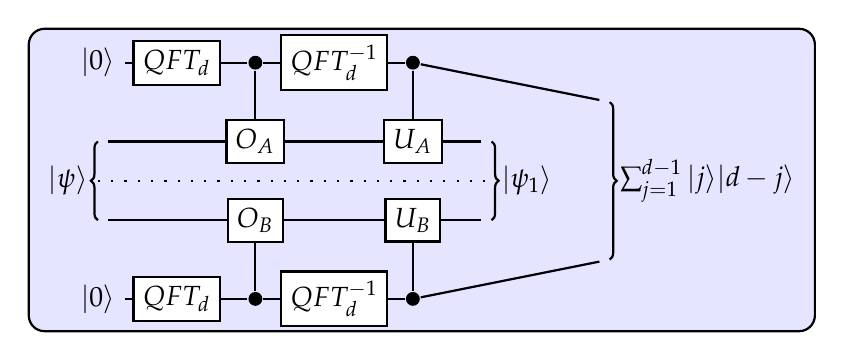
\begin{tikzpicture}[thick]
        %
        % `operator' will only be used by Hadamard (H) gates here.
        % `phase' is used for controlled phase gates (dots).
        % `surround' is used for the background box.
        \tikzstyle{operator} = [draw,fill=white,minimum size=1.5em] 
        \tikzstyle{phase} = [fill,shape=circle,minimum size=5pt,inner sep=0pt]
        \tikzstyle{surround} = [fill=blue!10,thick,draw=black,rounded corners=2mm]
        %
        % Bracket
        \draw[decorate,decoration={brace,mirror},thick] (0,-1) to
    	node[midway,left] (bracket1) {$\ket{\psi}$}
    	(0,-2);
        % Qubits
        \node at (0,0) (q1) {$\ket{0}$};
        \node at (0,-1) (q2) {};
        \node at (0,-2) (q3) {};
        \node at (0,-3) (q4) {$\ket{0}$};
        %
        % Column 1
        \node[operator] (op11) at (1,0) {$QFT_d$} edge [-] (q1);
        \node[operator] (op14) at (1,-3) {$QFT_d$} edge [-] (q4);
        %
        % Column 3
        \node[phase] (phase11) at (2,0) {} edge [-] (op11);
	\node[operator] (op22) at (2,-1) {$O_A$} edge [-] (q2);
	\node[operator] (op23) at (2, -2) {$O_B$} edge[-] (q3);
        \node[phase] (phase14) at (2,-3) {} edge [-] (op14);
        \draw[-] (phase11) -- (op22);
        \draw[-] (phase14) -- (op23);
        %
        % Column 4
        \node[operator] (op31) at (3,0) {$QFT_d^{-1}$} edge [-] (phase11);
        \node[operator] (op34) at (3,-3) {$QFT_d^{-1}$} edge [-] (phase14);
        %
        % Column 5
        \node[phase] (phase21) at (4,0) {} edge [-] (op31);
	\node[operator] (op42) at (4,-1) {$U_A$} edge [-] (op22);
	\node[operator] (op43) at (4, -2) {$U_B$} edge[-] (op23);
        \node[phase] (phase24) at (4,-3) {} edge [-] (op34);
        \draw[-] (phase21) -- (op42);
        \draw[-] (phase24) -- (op43);
        %
        % Column 6
        \node (end2) at (5,-1) {} edge [-] (op42);
        \node (end3) at (5,-2) {} edge [-] (op43);
        %
        % Bracket
        \draw[decorate,decoration={brace},thick] (5,-1) to
    	node[midway,right] (bracket) {$\ket{\psi_1}$}
    	(5,-2);
        %
        % Column 7
        \node (end1) at (6.5,-0.5) {} edge [-] (phase21);
        \node (end4) at (6.5,-2.5) {} edge [-] (phase24);
        % Dashed line
        \draw[loosely dotted] (0,-1.5) -- (5,-1.5);
        % Bracket
        \draw[decorate,decoration={brace},thick,] (6.5,-0.5) to
    	node[midway,right] (bracket2) {$\sum_{j=1}^{d-1}\ket{j}\ket{d-j}$}
    	(6.5,-2.5);
        %
        % Background Box
        \begin{pgfonlayer}{background} 
        \node[surround] (background) [fit = (q1) (op14) (bracket1)(bracket2)] {};
        \end{pgfonlayer}
        %
        \end{tikzpicture}
	\caption{The isometries $\Phi_{A,1} \x \Phi_{B,1}$.}
\end{figure}
Note that $QFT_d$ denotes the generalized Quantum Fourier Transform.
With the help of \cref{eq:decomp}, we can prove that
\begin{align*}
    \Phi_{A,1}\x\Phi_{B,1}(\ket{\psi}) \appd{O(d r^{d} \ep^{1/8})} \sqrt{d-1}\ket{\psi_1} \x \frac{1}{\sqrt{d-1}}\sum_{j=1}^{d-1} \ket{j}\ket{d-j}.
\end{align*}
This is the first application of the generalized swap-isometry \cite{yang2013} to a robust self-testing proof.  
Applying the second isometry to the state $\sqrt{d-1}\ket{\psi_1}$ gives us that
\begin{align*}
    \Phi_{A,2}\x\Phi_{B,2}(\sqrt{d-1}\ket{\psi})
    \appd{O(\sr \se)} \ket{junk} \x 
    \ket{EPR}^{\x 2}.
\end{align*}
Details about these two isometries can be found in
Section $6.4$ of the attached report.

In summary, 
for any $d \in D$, the maximally entangled state
of local dimension $4(d-1)$, $\frac{1}{\sqrt{d-1}} \sum_{j=1}^{d-1} \ket{j}\ket{d-j} \x \ket{EPR}^{\x 2}$, can be 
robustly self-tested by the correlation $\fC(d,r)$ 
where $r$ is the smallest primitive root of $d$.
Since $D$ has infinitely many elements and, for each $d$, 
its smallest primitive root is at most $5$, 
we have proved \cref{thm:inf}.


\textbf{Our contributions}:
We identify a family of correlations with constant-sized input and output alphabets that can be used to robustly self-test
maximally entangled states with unbounded local dimensions. Before our work, the most efficient way 
uses $O(\log d)$-sized input and $O(\log \log d)$-sized output alphabets to robustly self-test
the maximally entangled state of dimension $d = 2^n$ \cite{lowdegree}.  


Our result gives us deeper understandings of the set of quantum correlations.
In previous works that proved the non-closeness of the set of quantum correlations \cite{slofstra2017, slofstra2018}, 
lower bounds of the entanglement required to achieve certain correlations are identified.
We take a step further and discover a large family of correlations that we know exactly the entangled state
required to achieve each of the correlations in this family. 

It has been shown that robust self-testing allows a versifier to encode the verification of
a large computational problem into small questions \cite{fitzsimons2019,neexp}. One of the future applications of our result 
is to further reduce the lengths of questions for entanglement-assisted interactive proof systems.

\bibliographystyle{alphaurl}
\bibliography{quantum_correlation}
\end{document}